%%==================================================
%% chapter04.tex for BIT Master Thesis
%% modified by 朱杰
%%==================================================
\chapter{基于稳定标签传播的重叠社区发现算法}
在验证了上一章所提稳定策略在 LPA 算法上的有效性的基础上,将此稳定策略运用到 COPRA 算法中,以验证其在重叠社区发现算法中的有效性。COPRA 算法[?]和 SLPA 算法[?]通过允许每个节点拥有多个标签的方法,将 LPA 算法扩展应用于重叠社区的发现,它们既继承了 LPA 算法的优点,也保留了 LPA 算法不稳定和鲁棒性差等缺点。COPRA 算法是最早的基于标签传播的重叠社区发现算法。

本章提出一种基于稳定标签传播的重叠社区发现算法(Overlapping Community Detection Algorithm Based on Stable Label Propagation),下文简称 OCDABSLP。OCDABSLP 算法在迭代执行标签更新过程中,当节点属于所有社区的隶属度都小于阈值且最大值有多个时,选择隶属度最大的多个标签中标签影响强度最大的标签。满足终止条件后,算法根据节点的标签将其划分到相应社区中,拥有多个标签的节点被划分到相应的多个社区中,成为重叠节点,得到最终的重叠社区划分结果。在不同复杂网络数据集上的大量实验表明本章算法能够得到比现有的大部分算法更好的社区划分结果。

本章接下来的内容组织结构上将先简单介绍下多标签传播算法(COPRA),然后详细介绍OCDABSLP 算法的设计思路、核心思想和关键步骤等,最后在真实网络以及人工基准网络上的实验,并与其他基准算法进行对比实验,以此来分析算法的效果。

\section{多标签传播算法的缺陷分析}

Gregory 等人[?]提出的 COPRA 算法是第一个利用标签传播思想进行重叠社
区发现的算法。算法中每个节点可以以不同隶属度拥有多个标签,每个节点包含
一组标签-隶属度对$(l, b)$,$l $表示节点所属社区的编号,$b $表示节点属于该社区的
隶属程度,$b_t(l, i)$表示在第$ t $次标签传播结束时节点$ i $属于社区$ l $的隶属程度。
COPRA 通过迭代地更新各个节点的标签及隶属度来获取社区结构。

与 LPA 算法相同,初始时,COPAR 算法为每个节点分配一个各不相同的标
签,并将其隶属度设置为 1,即 $b_0(i, i) = 1$。然后采用同步更新策略进行标签更新
迭代,在每次更新过程中,用邻接点中出现的所有相同标签的平均隶属度更新该
节点的标签-隶属度对列表。每一轮更新后,删除隶属度小于 $\frac{1}{v}$ 的标签($v$ 是算法的参数),当一个节点的所有标签对应的隶属度都小于 $\frac{1}{v}$ 时,就只保留一个
隶属度最大的标签,若此时有多个标签的隶属度同时取最大值,就随机保留隶属
度最大的标签中的一个,然后对所有剩余标签的隶属度进行归一化。更新结束后,
算法根据节点的标签将其划分到相应的社区中。一个节点最后拥有的标签数即为
它被划分到的社区的个数。 

函数 $b_t(l, i)$用于计算在第 $t $次迭代中,节点$ i $属于社区$ l $的隶属程度,计算如
公式\ref{eqn:lishudu}所示。

\begin{equation}
  \label{eqn:lishudu}
  b_t(l,i)=\frac{\sum_{j\in \Gamma_i }b_{t-1}(l,j)}{d_i}
\end{equation}

COPRA 算法的执行过程如算法\ref{alg:COPRA}所示。

\begin{algorithm}[htb]  
  \caption{多标签传播算法(COPRA)}  
  \label{alg:COPRA}  
  \begin{algorithmic}[1]  
    \Require  
    复杂网络 $G = (V, E)$,最大迭代次数 $maxRun$   
    \Ensure  
      社区划分结果;  
    \State 初始化,为网络中的每个节点分配一个各不相同的标签,标签-隶属度对集合为${(i,l)}$;
    
          令迭代次数$t=0$;  

    \State 标签传播迭代过程:

    (a)如果迭代次数 $t > maxRun$,标签传播迭代过程结束,转 Step3;
    
    否则继续算法。 

    (b)对于每个节点$v_i\in V$,根据公式\ref{eqn:lishudu}计算该节点属于其邻接点集合中出现的所有标签的隶属度,更新标签-隶属度对列表。
    
    根据参数$v$删除不满足条件的标签,并对剩余标签进行归一化。 
     
    (c)如果连续两次迭代结束后,标签集合的大小不变,那么标签传播迭代过程停止,
    转Step3;
    
    否则,令$t = t+1$转到步骤(a)继续执行。

    \State 社区划分,将拥有相同标签的节点划分到同一个社区中,不同标签的种类就表示网络中社区的个数。
  \end{algorithmic}  
\end{algorithm} 

COPRA 算法继承了 LPA 算法的优点,也保留了 LPA 算法稳定性和鲁棒性差等缺点。 

\section{算法稳定性设计}
\subsection{标签初始化阶段的改进}
标签传播算法首先为网络中所有的节点分配一个
初始标签,然后对这些标签进行迭代更新,如果网络的 节点很多, 那么更新所有这些标签的时间空间开销就 会增大,考虑到在网络中有很多节点的度数较小,它们 的更新完全依赖于它们邻节点的标签, 可以采用较少 初始化标签的量来节省开销和算法的不稳定性。 我们提出节点度数 $d_0$($d_0$ 为自然数)这一阈值,对节点度数 小于 $d_0$ 的节点,其节点标签不予考虑,这样便大大减少了初始化标签的数目,也减少了此类节点的更新量,降 低了更新复杂度。至于 $d_0$ 的取值问题,可以结合网络情况,以及实验结果得出最佳阈值。

\subsection{标签选择阶段的改进}
原始COPRA算法中的唯一一个不稳定因素是当节点属于所有社区的隶属度
都小于阈值且最大值有多个时,会随机选择一个标签。因此,在此处对 COPRA
算法进行改进。当出现上述情形时,选择隶属度最大的多个标签中标签影响强度
最大的标签。当标签影响强度最大的标签仍有多个时,保留所有标签影响强度最
大的标签。标签影响强度的计算如公式\ref{eqn:LI2}所示。

\begin{equation}
  \label{eqn:LI2}
  NI(i,l)=\sum_{j \in \Gamma _i} b_{t-1}(l,j) \frac{NI(j)}{d_j}
\end{equation}

\section{算法执行步骤}
OCDABSLP 算法的主要步骤包括初始化、迭代标签传播和社区划分。图\ref{fig:fig4-1}
为 OCDABSLP 的算法流程图。

\begin{figure}
  \centering
  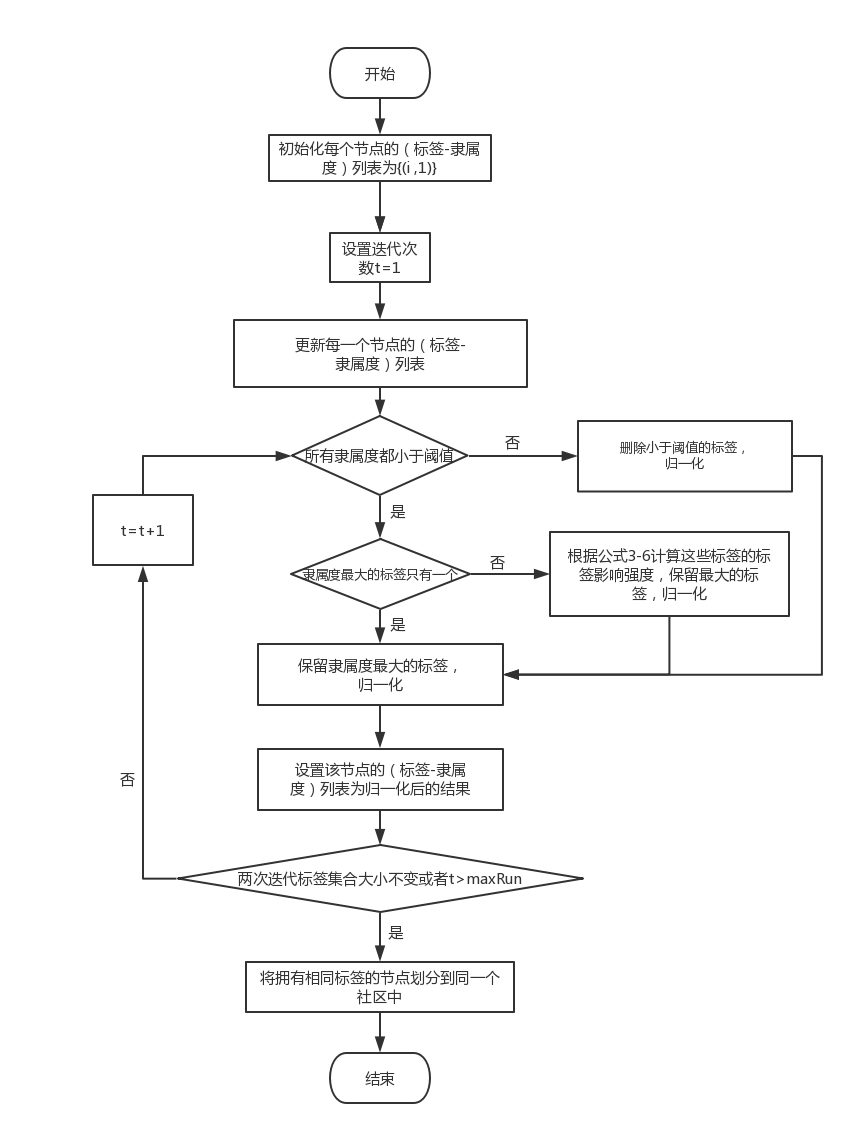
\includegraphics[width=1\textwidth]{figures/fig4-1}
  \caption{OCDABSLP算法流程图}\label{fig:fig4-1}
\end{figure}

通过一个简单的例子来展示 OCDABSLP算法的执行过程,如图\ref{fig:fig3-4}所示,算法
中参数$\alpha =1$。图中每一个圆圈代表一个节点,节点间的连线代表节点间的边,
节点外的实数表示节点的影响值$ NI$。按节点影响值降序排列图中的节点$v_1-v_2-v_4-v_6-v_5$
(当节点影响值相同时,按节点的先后顺序排列),以该顺序作为
节点更新的顺序,标签更新过程如图\ref{fig:fig3-4}所示。

\begin{figure}
  \centering
  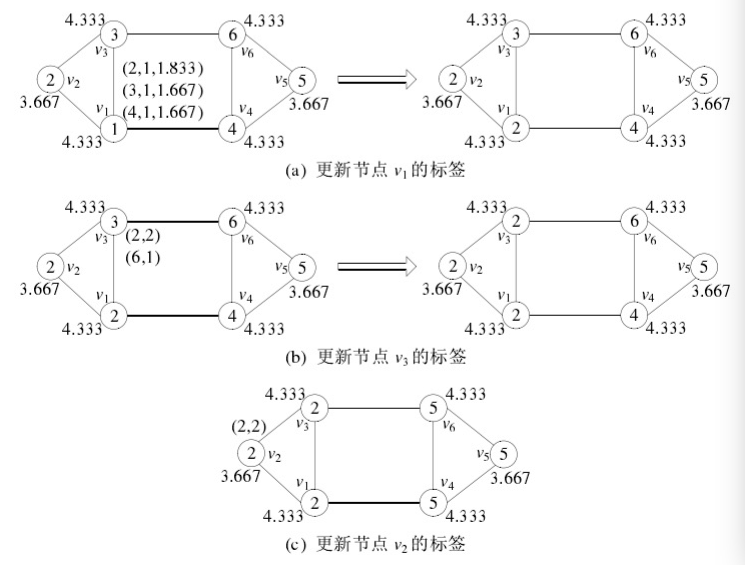
\includegraphics[width=0.75\textwidth]{figures/fig3-4}
  \caption{OCDABSLP算法标签传播过程示意图}\label{fig:fig3-4}
\end{figure}

 按照节点更新顺序,第一个更新节点$v_1$
的标签。首先为节点$v_1$计算一系列
的三元组$(l,|\Gamma _1^l|,LI(v_1,l))$,其中$ l $表示其邻接点中包含的标签,
$|\Gamma _1^l|$表示标签为
$l $的邻接点的个数,最后一项$LI(v_1,l)$表示标签对该节点的影响强度,该项是一个
可选项,当不能通过传统的标签选择策略得到一个确定的标签时,通过公式\ref{eqn:LI}
计算得到。如图\ref{fig:fig3-4}(a)所示,节点$ v_1
$有三个邻接点$ v_2$
、$v_3$和 $v_4$,并且它们的标签
各不相同,计算得到节点 $v_1$
对应的三元组集合为${(2, 1, 1.833), (3, 1, 1.667), (4, 1, 
1.667)}$。因此选择标签 2 作为节点 $v_1$
的新标签。 

接着更新节点 v3的标签。更新完节点 $v_1$的标签之后,如图\ref{fig:fig3-4}(a)右图所示,节点$ v_3$共有三个邻接点$ v_1$、$v_2$和$ v_6$,其中$ v_1$和$ v_2$的标签相同,均为标签 2,只有节点 $v_6$的标签不同。因此选择标签 2 作为节点 $v_3$的新标签,如图\ref{fig:fig3-4}(b)所示。接下来节点$ v_4$和$ v_6$标签的更新分别与节点$ v_1$和$ v_3$的情况相同,更新结果如图\ref{fig:fig3-4}(c)所示。

最后只有节点$ v_2$和$ v_5$没有更新,此时如图\ref{fig:fig3-4}(c)所示,节点 $v_2$和它的邻接点的标签都为标签 2,而节点 $v5$与它所有的邻接点的标签都为标签 5,因此节点$v_2$和$ v_5$的标签不需要改变。

通过执行 OCDABSLP 算法,在该网络上仅需执行一次标签更新过程就得到了最
终稳定的社区划分结构,得到两个与真实情况一致的社区。由于算法的执行过程
中没有了随机因素的存在,因此算法的输出结果是确定的且优质的。 

\section{算法时间复杂度分析}
OCDABSLP 算法的时间复杂度分析如下: 

(1)为每个节点初始化标签所用时间复杂度为$ O(|V|)$; 

(2)每次标签传播过程分为两部分: 传统的标签传播过程:$O(v|E|log(v|E|/|V|))$;当节点属于所有社区的隶属度都小于阈值且最大值有多个时,利用
公式\ref{eqn:LI2}计算标签影响值的过程:$O(v|E|log(v|E|/|V|))$; 

(3)将相同标签的节点划分到一个社区的时间复杂度为 $O(|V|)$。 

标签传播过程是不断迭代执行的,因此整个算法的时间复杂度为
$2O(|V|)+2tO(v|E|log(v|E|/|V|))$。

\section{验证实验}
本节为本章提出的基于稳定标签传播的重叠社区发现算法OCDABSLP算法进行实验验证。首先介绍实验的软硬件环境和采用的数据集,然后对算法的评价指标进行简单阐述,最后是相关对比实验的结果展示与分析。

\subsection{实验环境}
本文实现的OCDABSLP算法所使用的软硬件环境与上一章节的CDABSLP算法一致,机器配置如表\ref{tab:tab3-1}所示。OCDABSLP算法使用Python语言编程实现,均基于Python的复杂网络相关软件包Networkx,使用Anaconda来对软件包进行管理和部署,具体配置如表\ref{tab:tab3-2}所示。

\subsection{数据集}
选用4组不同的LFR基准网络人工生成数据集进行实验验证本章所提算法的有效性。 

(2)LFR人工基准网络

LFR基准网络是目前在社区发现领域使用最多的人工数据集之一。通
过调整网络生成参数可以产生用户需要的不同的人工数据集,LFR 基准网络的主
要生成参数及其含义在上一章节中已经提及,如表\ref{tab:tab3-4}所示。

本节实验将生成四组具有重叠社区结构的 LFR 基准网络数据集,详细的生成参数如
表\ref{tab:tab4-1}示。 

\begin{table}
  \centering
  \caption{四组重叠LFR基准网络生成参数} \label{tab:tab4-1}
  \begin{tabular*}{0.9\textwidth}{@{\extracolsep{\fill}}ccccccccc}
  \toprule
    编号		&N  &avgk &maxk &minc &maxc &mu &on &om\\
  \midrule
    S7	&100000  &150 &5000 &100 &5000 &0.1 &1000 &$2\sim 8$\\
    S8 &100000  &150 &5000 &100 &5000 &0.3 &1000 &$2\sim 8$\\
    S9 &500000  &150 &5000 &200 &10000 &0.1 &1000 &$2\sim 8$\\
    S10 &500000  &150 &5000 &200 &10000 &0.3 &1000 &$2\sim 8$\\
  \bottomrule
  \end{tabular*}
\end{table}

\subsection{评价指标}
本章采用重叠 NMI(ENMI)[?]和重叠模块度 EQ
[?]作为重叠社区发现结果的评价指标。下面介绍这些指标。

(1)EQ

在上一章节已经提到了模块度的概念,而重叠社区模块度(EQ)[?]可以在其公式\ref{eqn:modular}的基础上修改为公式\ref{eqn:modular2}。

\begin{equation}
  \label{eqn:modular2}
  Q=\frac{1}{2m} \sum_{k=1}^c \sum_{i,j \in C_k} \frac{1}{O_iO_j} \left [ A_{ij}-\frac{k_ik_j}{2m} \right ]  
\end{equation}

在公式\ref{eqn:modular2}中,i和j表示网络中的两个节点,m表示网络中边的数量,$k_i$和$k_j$表示节点i和j的度数,$O_i$和$O_j$表示节点i和j所属的社区的个数,A表示网络的邻居矩阵,$C_k$表示网络的第k个社区。该公式的数学意义为:网络中同一社区内部的边的比例与在同样社区结构下的基准网络内部边的比例的期望值之差。模块度越高,则网络中社区划分结果越好。


(2)ENMI

在上一章节已经提到了NMI的概念,而ENMI[?]是在其重叠社区上的扩展,具体计算方式详见公式\ref{eqn:enmi}。

\begin{equation}
  \label{eqn:enmi}
  NMI(X,Y) = 1 – \frac{1}{2} [H(X|Y)_{norm} + H(Y|X)_{norm}]
\end{equation}

其中$H(X,Y)$函数表示联合熵,X和Y分别是一个社区,$H(X \mid Y)$函数表示条件熵。

\subsection{实验结果及分析}

(1)人工基准网络上的实验

为了验证本章提出的稳定策略用在 COPRA 算法中的效果,进行本组实验,
将 OCDABSLP 算法与 COPRA 算法进行比较。图\ref{fig:S7ENMI}$\sim$\ref{fig:S10ENMI}中的八幅图分别是
OCDABSLP 算法和 COPRA 算法在四组重叠 LFR 基准网络数据集(S7$\sim$S10)上
实验结果的 ENMI 和 EQ 指标的对比图。实验中,参数 v 设置为 om 的值。由于
COPRA 算法存在随机性,因此取 10 次实验的平均值作为最后的结果。横轴代
表重叠节点所属的社区个数 om,取值从 2 到 8;左侧四幅图的纵轴代表社区划
分结果的 ENMI 值,右侧四幅图的纵轴表示实验结果的 EQ 值。 

\begin{figure}
  \centering
  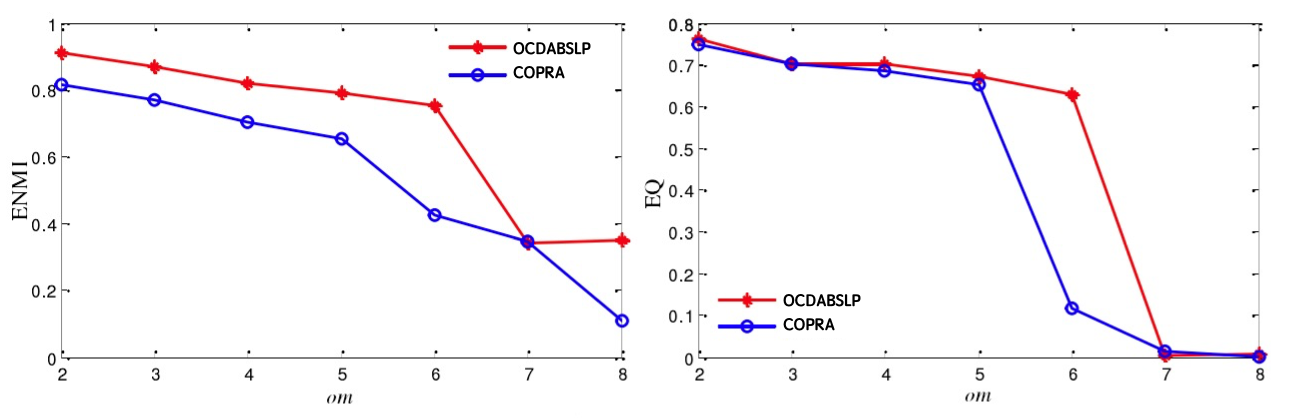
\includegraphics[width=0.75\textwidth]{figures/S7ENMI}
  \caption{在S7网络上的实验结果的ENMI和EQ比较}\label{fig:S7ENMI}

  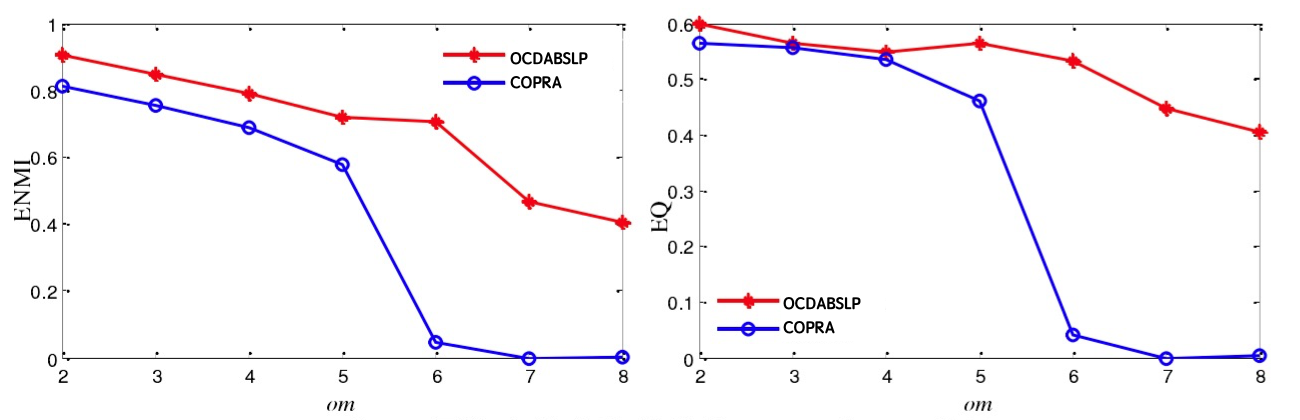
\includegraphics[width=0.75\textwidth]{figures/S8ENMI}
  \caption{在S8网络上的实验结果的ENMI和EQ比较}\label{fig:S8ENMI}

  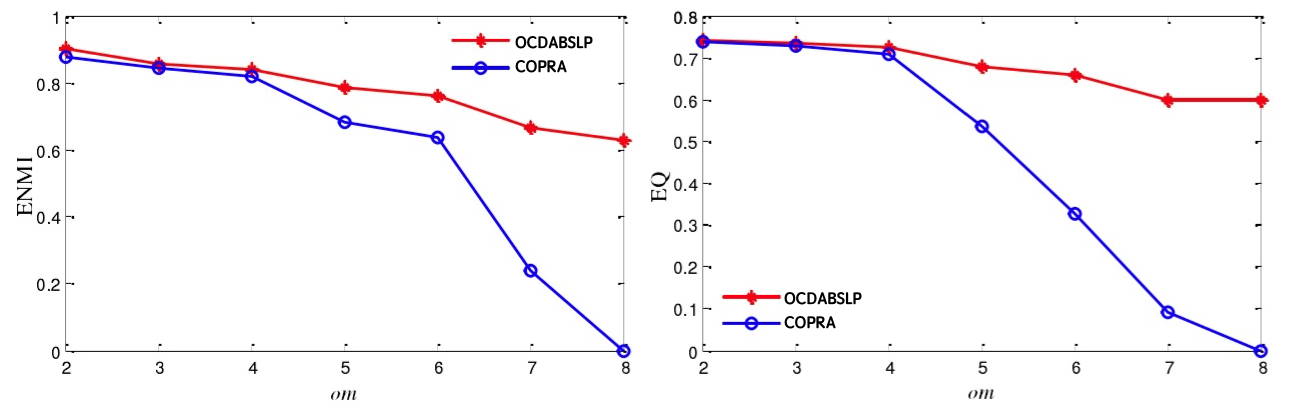
\includegraphics[width=0.75\textwidth]{figures/S9ENMI}
  \caption{在S9网络上的实验结果的ENMI和EQ比较}\label{fig:S9ENMI}

  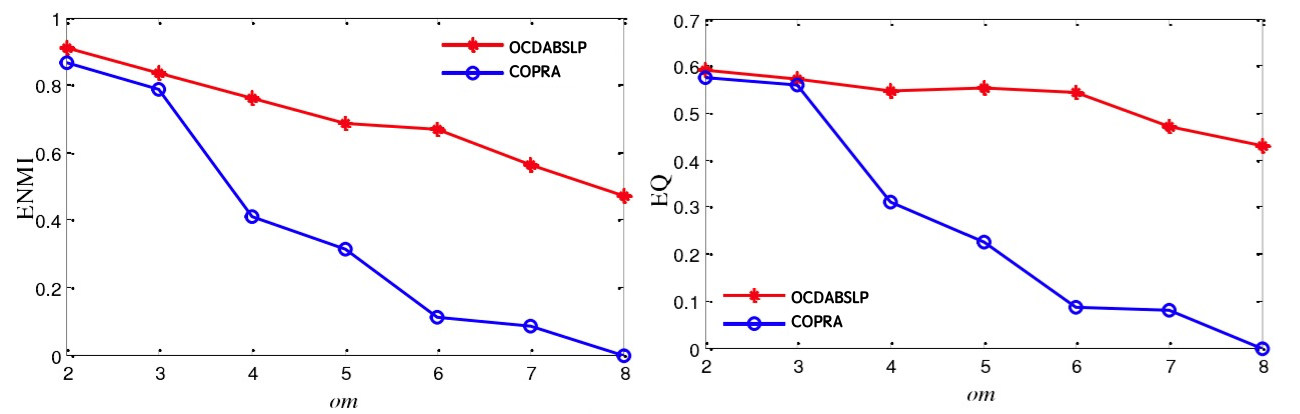
\includegraphics[width=0.75\textwidth]{figures/S10ENMI}
  \caption{在S10网络上的实验结果的ENMI和EQ比较}\label{fig:S10ENMI}

\end{figure}

从图\ref{fig:S7ENMI}$\sim$\ref{fig:S10ENMI}中可以看出,ODABSLP 算法不仅能够得到稳定的社区发现结果,
而且得到的社区结构 ENMI 和 EQ 两个指标都优于 COPRA 算法。验证了本章所
提方法在重叠社区发现方面能得到比较好的结果。

(2)可视化对比

待加入。。。


% \subsection{实验总结}

% OCDABSLP 算法采用同步更新策略,在标签更新过程中,当一个节点拥有
% 的所有标签对应的隶属度都小于 1/v,且此时有多个标签的隶属度同时取最大值
% 时,将节点影响值引入到标签隶属度计算公式中,得到这些标签的影响强度,保
% 留影响强度最大的标签,取代传统 COPRA 算法随机保留其中一个标签的方法,
% 提高算法的稳定性。在重叠 LFR 数据集上的实验结果表明 OCDABSLP 算法解决
% 了 COPRA 算法不稳定的问题,能够检测得到较优的重叠社区结构,验证了本章
% 提出的稳定策略在重叠社区发现算法 COPRA 算法中的适用性。

\section{本章小结}
本章小结内容凑字数本章小结内容凑字数本章小结内容凑字数本章小结内容凑字数本章小结内容凑字数本章小结内容凑字数本章小结内容凑字数本章小结内容凑字数本章小结内容凑字数本章小结内容凑字数本章小结内容凑字数本章小结内容凑字数本章小结内容凑字数本章小结内容凑字数本章小结内容凑字数本章小结内容凑字数本章小结内容凑字数本章小结内容凑字数本章小结内容凑字数本章小结内容凑字数本章小结内容凑字数本章小结内容凑字数本章小结内容凑字数本章小结内容凑字数本章小结内容凑字数本章小结内容凑字数本章小结内容凑字数本章小结内容凑字数本章小结内容凑字数本章小结内容凑字数本章小结内容凑字数本章小结内容凑字数本章小结内容凑字数本章小结内容凑字数本章小结内容凑字数本章小结内容凑字数本章小结内容凑字数本章小结内容凑字数本章小结内容凑字数本章小结内容凑字数本章小结内容凑字数本章小结内容凑字数